\newpage
\section{Versuchsaufbau und -durchführung}
        Der Aufbau des Versuches ist in Abbildung \ref{fig:Aufbau} zu sehen und kann in einen Abschnitt zur Anregung der Photolumineszenz und einen zu derer Detektion unterteilt werden. 
        \begin{figure}[h]
          \centering
          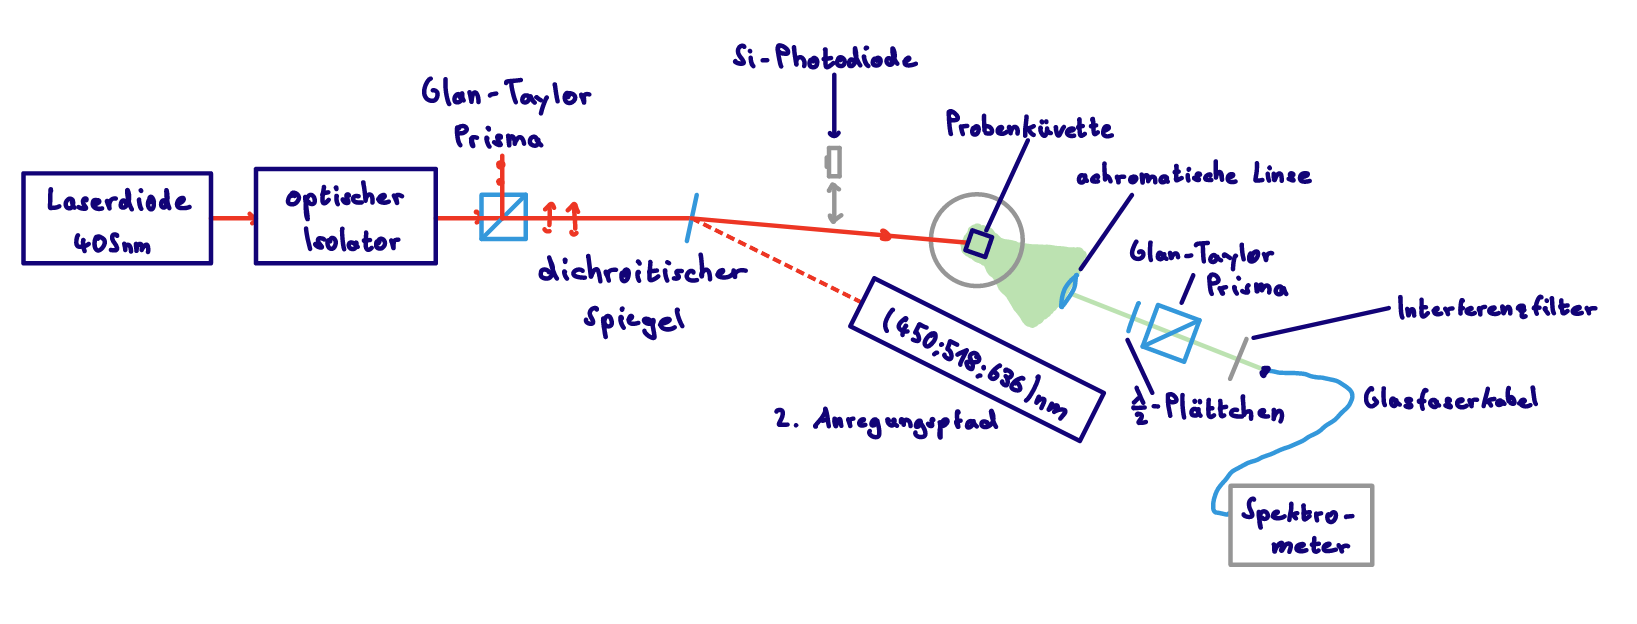
\includegraphics[width = 1\textwidth]{pictures/PL_Aufbau.png}
          \caption{Der Aufbau zur Vermessung der Photolumineszenz der verschiedenen Proben.}
          \label{fig:Aufbau}
        \end{figure}

        Der Anregungsabschnitt besteht aus dichroitischem Spiegel, der Licht mit einer Wellenlänge über \SI{425}{\nano\metre} reflektiert und Licht mit einer höheren Wellenlänge transmittiert. Dieser Spiegel 
        wird einseitig mit einem Diodenlaser der Wellenlänge \SI{405}{\nano\metre} bestrahlt, dessen Licht durchläuft einerseits einen optischen Isolator, um eine Rückreflexion in den Diodenlaser zu verhindern 
        und wird andererseits durch eine Glan-Taylor-Prisma in seiner Polarisation definiert. Dieser Laserstrahl wird gemäß der obigen Beschreibung durch den dichroitischen Spiegel direkt in Richtung Probe
        transmittiert. In einem zweiten Anregungspfad können drei weitere Laser der Wellenlängen \SI{450}{\nano\metre}, \SI{518}{\nano\metre} und \SI{636}{\nano\metre} platziert werden, deren Licht vom 
        dichroitischen Spiegel wiederum auf die Probenküvette reflektiert wird. Hinter dem dichroitischen Spiegel kann eine Si-Photodiode platziert werden, um die Anregungsleistung des Lasers zu messen.
        Es werden 4 Proben benutzt. 3 Proben sind CdSe-Nanokristalle unterschiedlicher Größe und eine Probe enthält Kohlenstoff-Nanopartikel.
        Im Detektionsabschnitt wird die durch Anregung der Proben entstehende Photolumineszenz-Strahlung \ref{fig:PL} zunächst durch eine achromatische Linse mit einer Brennweite von \SI{60}{\milli\metre} 
        kollimiert. Zur Untersuchung der Polarisation der Photolumineszenz wird ein $\lambda$/2-Plättchen mit einem Glan-Taylor-Prisma kombiniert, sodass nur eine ausgewählte Polarisation des kollimierten 
        Lichts transmittiert wird. Zuletzt wird die Strahlung des \SI{405}{\nano\metre}-Lasers über einen Interferenzfilter ausgefiltert und die verbleibende Strahlung per Glasfaserkabel in ein Spektrometer 
        eingekoppelt.
        \newpage
        Nachdem der Strahl justiert worden ist, werden zunächst alle Proben mit dem \SI{405}{\nano\metre}-Laser und einer Leistung von \SI{1}{\milli\watt} angeregt und die zugehörige Photolumineszenz 
        in Abhängigkeit der Polarisation dieser per Spektrometer vermessen.

        Anschließend wird die Photolumineszenz der ersten Probe bei Bestrahlung durch \SI{405}{\nano\metre}-Laser für Anregungsleistungen zwischen \SI{1}{\milli\watt} und \SI{20}{\milli\watt} in Schritten
        von ungefähr \SI{1}{\milli\watt} unabhängig von der Polarisation per Spektrometer vermessen.

        Zuletzt werden die Photolumineszenzspektren aller vier Proben bei Anregung mit den vier verschiedenen Laserwellenlängen erneut unabhängig von der Polarisation aufgenommen. 

        \FloatBarrier

        \begin{figure}[h]
          \centering
          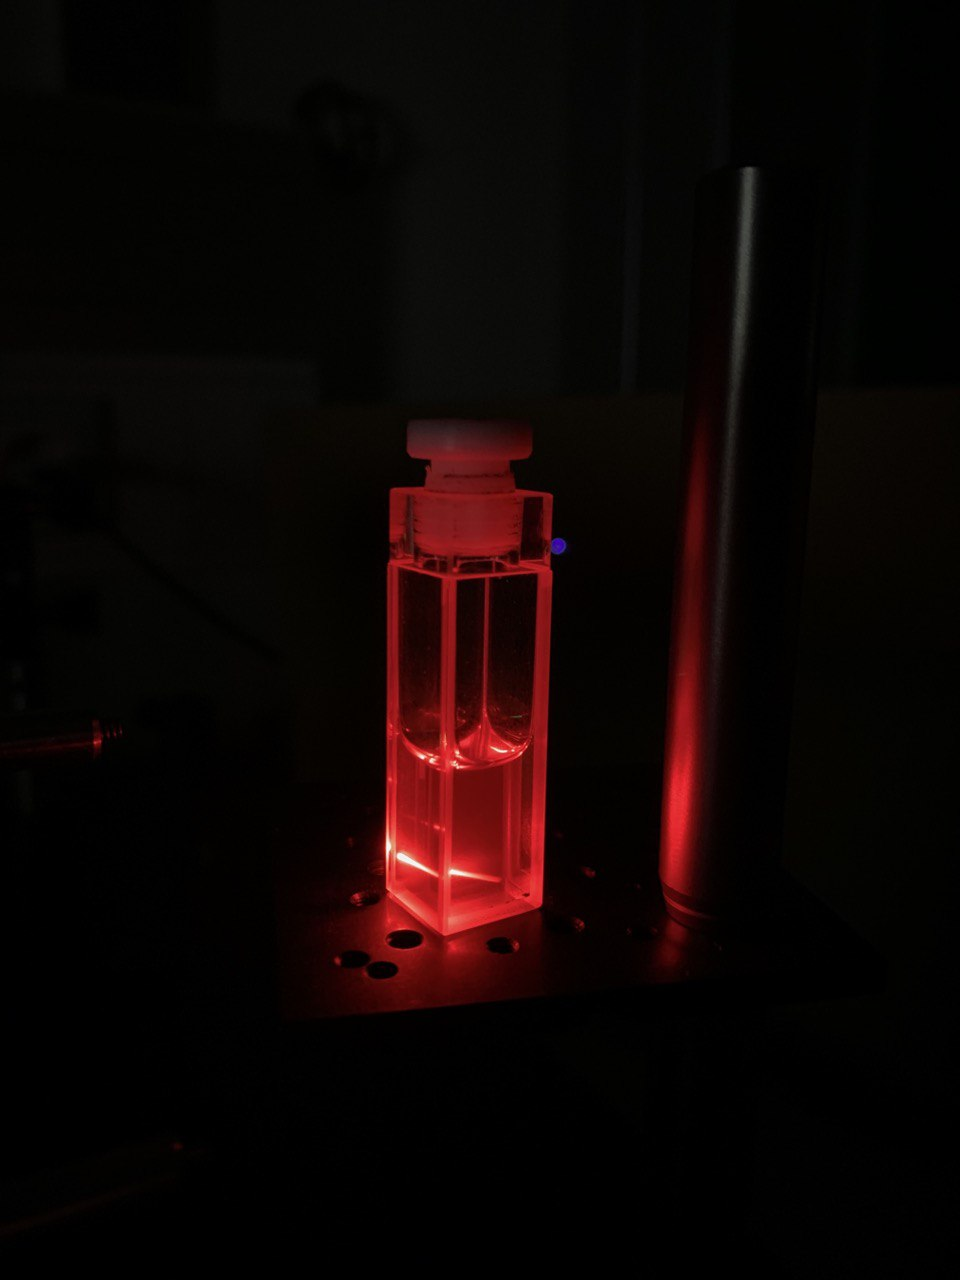
\includegraphics[width = 0.3\textwidth]{pictures/PL1.jpg}
          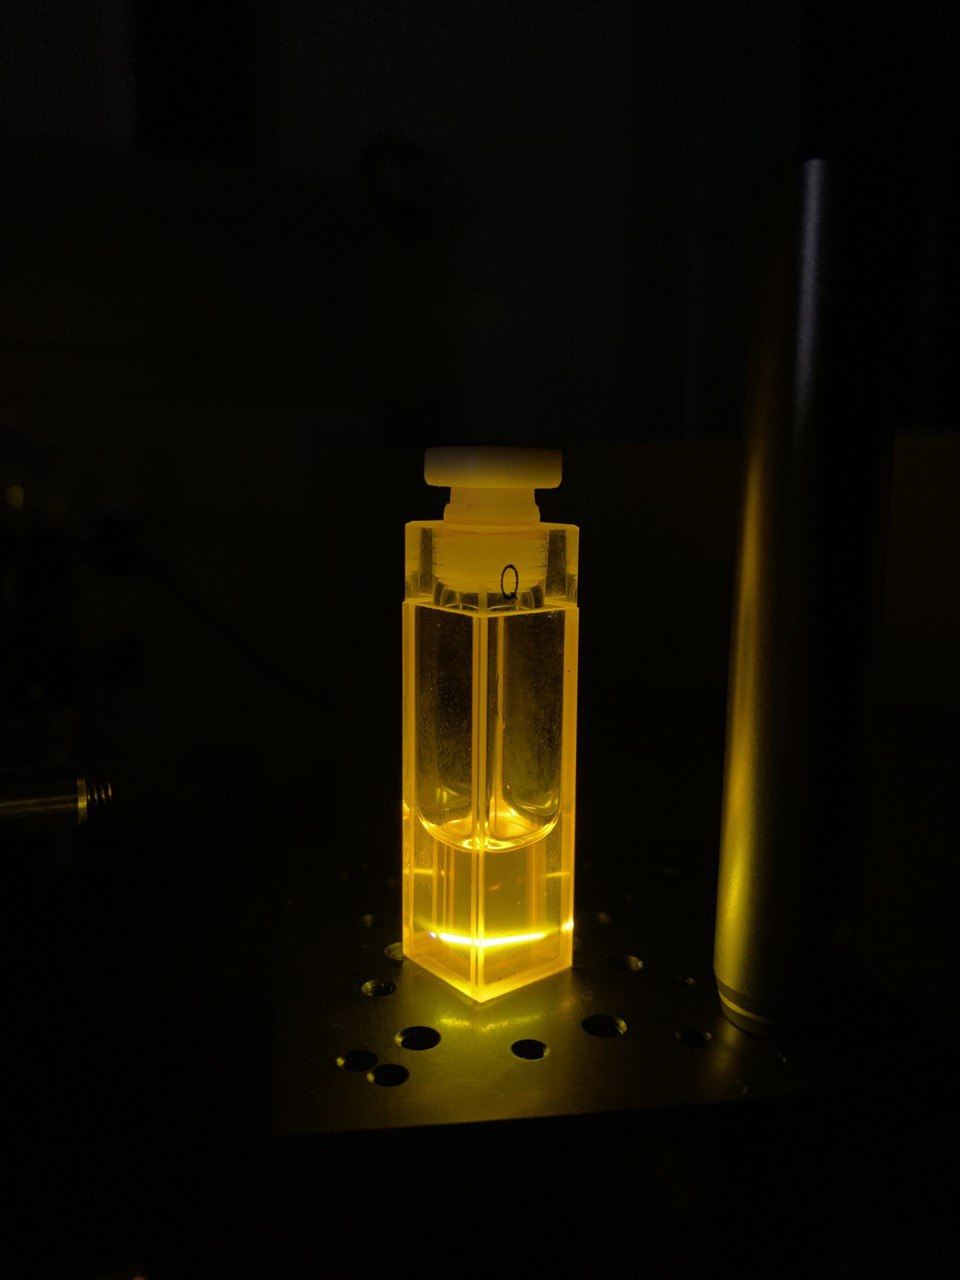
\includegraphics[width = 0.3\textwidth]{pictures/PL2.jpg}
          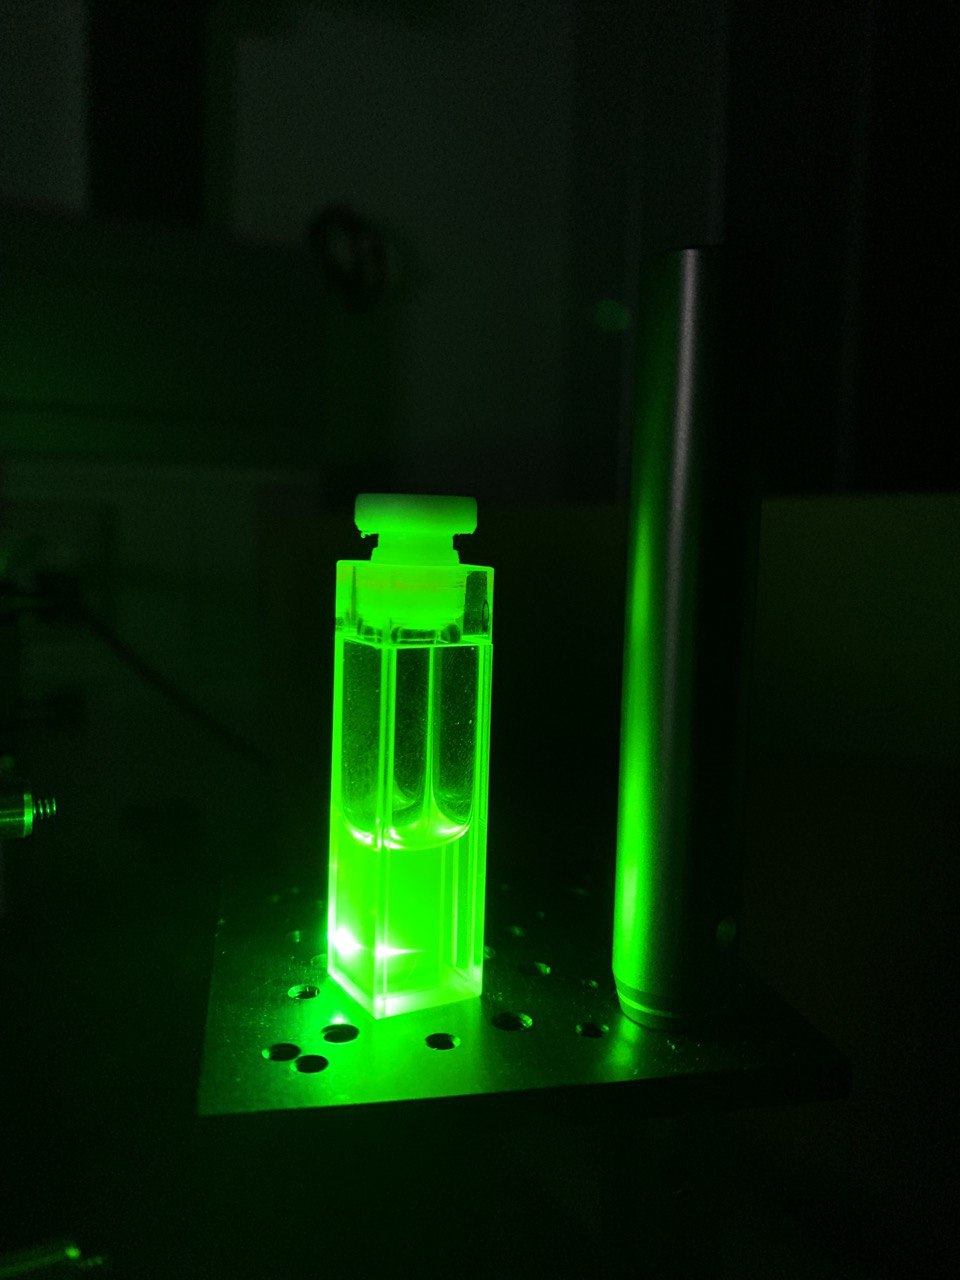
\includegraphics[width = 0.3\textwidth]{pictures/PL3.jpg}
          \caption{Die Photolumineszenz drei verschiedener Proben.}
          \label{fig:PL}
        \end{figure}

        \FloatBarrier